\documentclass{article}
\usepackage{Sweave}
\usepackage{tabularx}
\usepackage{geometry}
\geometry{margin=.5in}
\usepackage{enumerate}
\usepackage{graphicx}
\usepackage{subcaption}
\makeatletter
\setlength{\@fptop}{0pt}
\makeatother
\begin{document}
\Sconcordance{concordance:figures_page.tex:figures_page.Rnw:%
1 57 1}

%updated July 30 2018

%figure 1
\begin{figure}[ht!]
    \captionsetup{justification=centering}
    \begin{minipage}{\linewidth}
\subcaptionbox{Fraxinus excelsior}{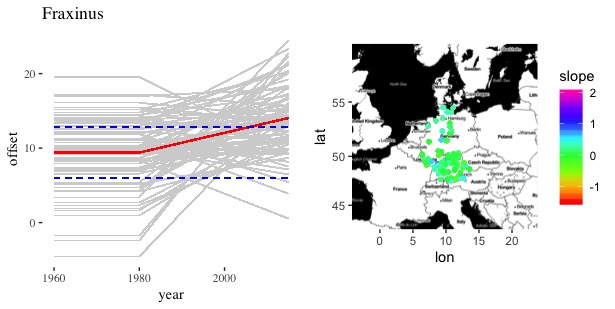
\includegraphics[width=\linewidth]{../figure/Fraz_hing_delta_fig1.jpeg}}

\subcaptionbox{Aesculus hippopotomus}{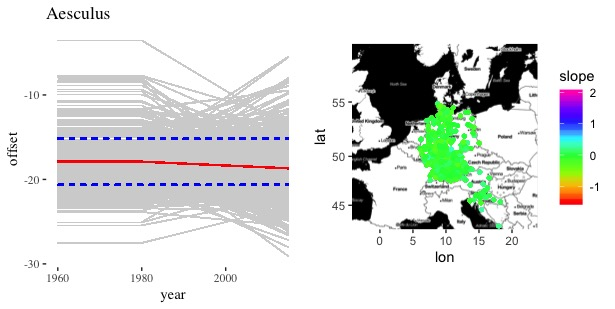
\includegraphics[width=\linewidth]{../figure/Aes_hing_delta_fig1.jpeg}}
    \end{minipage}
    \caption{FLS is changing with climate change, but this response is species specific, and the direction and strength of the change is real variable}
\end{figure}

%figure 2
\begin{figure}[ht!]
    \captionsetup{justification=centering}
    \begin{minipage}{\linewidth}
\subcaptionbox{Quercus rubra}{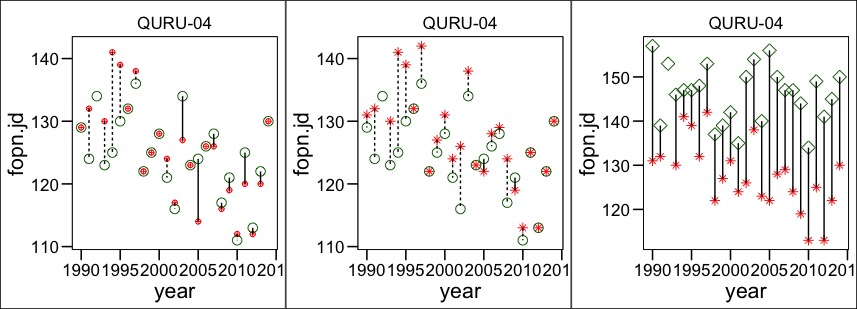
\includegraphics[width=\linewidth]{../figure/Quercus4_HF_fig2.jpeg}}

\subcaptionbox{Fraxinus americana }{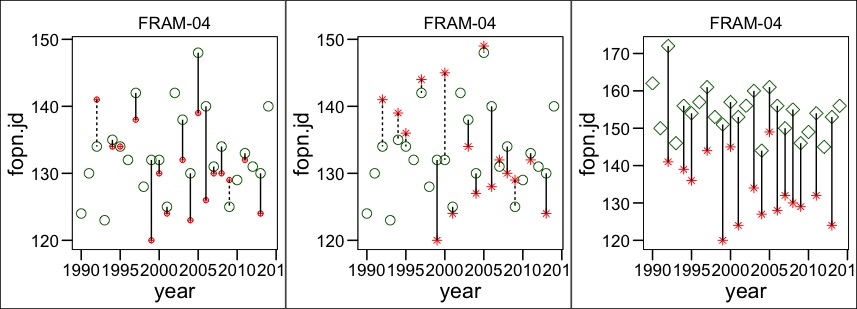
\includegraphics[width=\linewidth]{../figure/Fraxinus4_HF_fig2.jpeg}}
    \end{minipage}
    \caption{Variability for 3 classifications FLS for individuals at harvard forest 1990-2015.}
\end{figure}

\begin{figure}[ht!]
    \captionsetup{justification=centering}
    \begin{minipage}{.6\linewidth}
\subcaptionbox{MTSV}{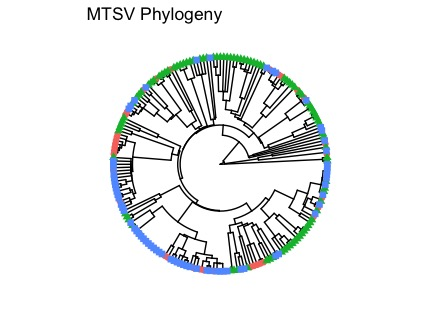
\includegraphics[trim=3cm 1cm 3cm 1.5cm, clip=true]{MTSV_phylo_nolabs.jpeg}}\subcaptionbox{USFS}{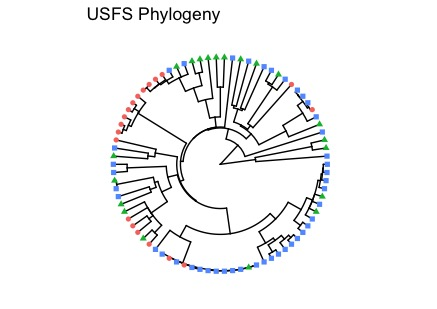
\includegraphics[trim=3cm 1cm 3cm 1.5cm, clip=true]{USFS_phylo_nolabs.jpeg}}
    \end{minipage}
    \caption{They phylogenies for MTSV and USFS data coded by FLS classification.}
\end{figure}




\begin{figure}[!tbp]
  \centering
 \fbox{ 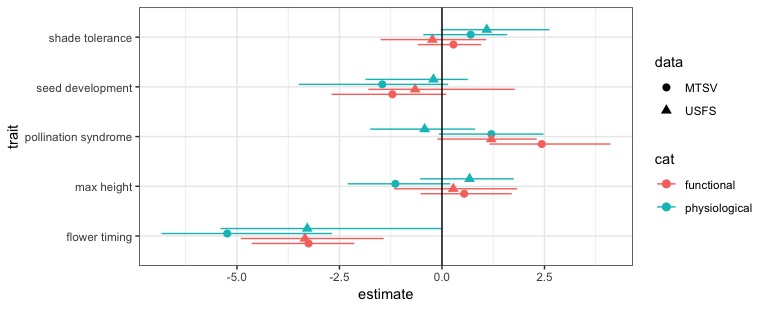
\includegraphics[width=\textwidth]{Data_comparision_plot.jpeg}\label{fig:f7}}
\caption{Golly, we get different outputs.}
\end{figure}




\end{document}
